% 独立章节文件：可单独编辑，统一由 main.tex 引入。
\chapter{系统组成、通信与安全约束}
\section{设备架构}
\begin{figure}[H]\centering
\begin{tikzpicture}[>=Stealth,node distance=10mm and 9mm, every node/.style={font=\small},box/.style={draw=border,fill=soft,rounded corners=2mm,align=center,minimum height=12mm,text width=33mm},top/.style={draw=teal,fill=teal!8,rounded corners=2mm,align=center,minimum height=13mm,text width=37mm}]
\node[top] (app) {Python / PySide6\\自动实验调度};
\node[box,below left=12mm and 19mm of app] (imu) {ASM330LHHX\\串口 / MCU / Modbus};
\node[box,below=12mm of app] (turn) {2TD600 或 2FDT600WK\\分别使用对应驱动};
\node[box,below right=12mm and 19mm of app] (chamber) {Snap7 / PLC 温箱\\SP / PV / 状态 / 报警};
\node[box,below=15mm of turn,text width=65mm] (alg) {质量筛选与统一工况记录\\常温 A/B/C / 温补 $\mathbf F(T),\vect b(T)$ / 报告};
\draw[->,thick,blue] (app)--(imu);\draw[->,thick,blue] (app)--(turn);\draw[->,thick,blue] (app)--(chamber);
\draw[->,thick,teal] (imu.south)--(alg.north west);\draw[->,thick,teal] (turn)--(alg);\draw[->,thick,teal] (chamber.south)--(alg.north east);
\end{tikzpicture}
\caption{当前上位机的控制与计算链路示意；设备型号必须由对应页面明确选定。}
\end{figure}


\section{转台型号必须隔离}
\noindent\begin{tabularx}{\linewidth}{@{}p{31mm}p{34mm}Y@{}}\toprule
设备 & 工程接口 & 实际用途\\\midrule
2TD600 & \Code{2TD600.dll} & 原常温 ACC/GYRO 自动标定任务。\\
2FDT600WK & \Code{2FDT600WK.dll} & 温控转台：双轴姿态/正反速率；两个独立轴系。\\
温箱 PLC & \Code{python-snap7} + 原温箱驱动 & 定值模式、SP 写入、PV/SP 回读、运行状态和报警读取。\\\bottomrule\end{tabularx}
如洋手册规定 2FDT600WK 运动单元使用 RS-422 通信，两轴独立测控；温箱规格列有 RS-232 二次开发接口。\textbf{现场已用过的原 PLC 设温、读温控制路径}是当前集成版的首选；不代表任意其他温箱可以直接复用相同 PLC 寄存器。\source{如洋说明书第 4、7、10、13 页；原温控驱动。}

\section{如洋 2FDT600WK 主要参考能力}
\noindent\begin{tabularx}{\linewidth}{@{}p{49mm}Y@{}}\toprule
项目 & 说明书标称值\\\midrule
内环角速度范围 & $\pm0.001$ 至 $\pm200^\circ/\mathrm{s}$\\
外环角速度范围 & $\pm0.001$ 至 $\pm100^\circ/\mathrm{s}$\\
角位置定位精度 & 两轴各 $\pm3$ 角秒\\
温箱标称范围 & $-40$ 至 $+105\, ^\circ\mathrm C$\\
温度偏差 / 波动 / 均匀度 & $\pm2\, ^\circ\mathrm C$ / 不超过 $\pm1\, ^\circ\mathrm C$ / 不大于 $\pm2\, ^\circ\mathrm C$\\
运动通信 & RS-422，115200 bps（协议附件 1）\\\bottomrule\end{tabularx}
上述是\textbf{硬件说明书能力}，不是当前软件的自动指令限幅；当前温补动态工况另有限定不超过 $5^\circ/\mathrm{s}$，不能因说明书最大转速较高而绕过现有安全检查。

\section{启动前安全检查清单}
\begin{enumerate}
\item 机械固定和配平；活动区域无障碍；旋转时机械锁必须处于松开状态；硬件急停可用。
\item 核对内外轴身份、正向、找零状态、重力向量和装夹坐标，不得将 2TD600 与 2FDT 接口混用。
\item 温箱门、线束、旋转余量、被测样品工作温度及其凝露风险按现场规程确认。
\item MCU 加速度/陀螺量程、ODR、数据比例、供电状态在整轮实验中保持不变。
\item 自动试验中任何反馈超时、伺服故障、PLC 报警、丢帧、温度异常时均进入受控中止；软件无法确认停车时\textbf{立即转人工硬件急停处置}。
\end{enumerate}


\section{设备外观与双轴机构（原厂图示）}
\begin{notice}
以上照片与示意图用于识别设备结构，\textbf{不等于运动空间防碰撞验证}。自动工况必须使用经过现场确认的坐标映射和机械安全限制。
\end{notice}
\begin{figure}[H]
\centering
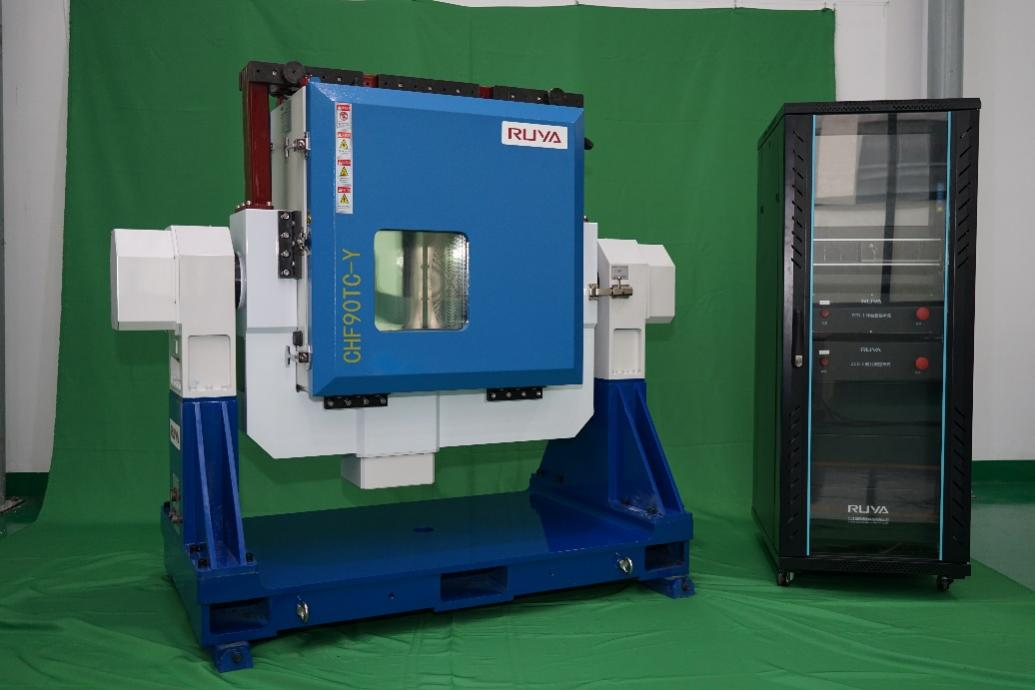
\includegraphics[width=.64\textwidth,keepaspectratio]{assets/photos/ruya_2fdt600wk_system.jpeg}
\caption{如洋 2FDT600WK 双轴温控转台整体外观；图片摘自用户提供的原厂使用说明书第 1 章。}
\label{fig:ruya-system}
\end{figure}
\begin{figure}[H]
\centering
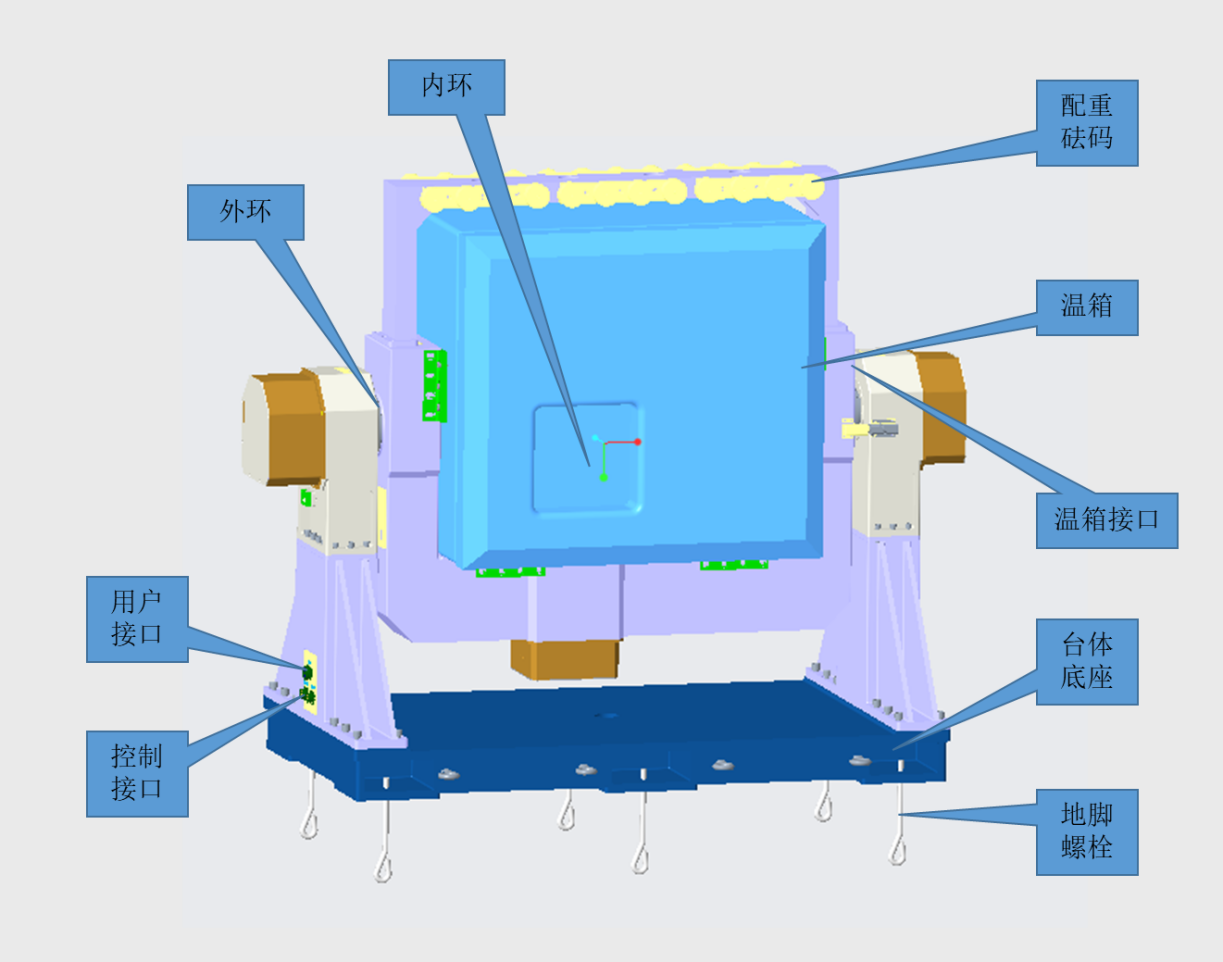
\includegraphics[width=.68\textwidth,keepaspectratio]{assets/schematics/ruya_2fdt600wk_mechanism.png}
\caption{2FDT600WK 台体结构示意图；正式试验的内外框轴正方向应以现场复核记录为准。}
\label{fig:ruya-mechanism}
\end{figure}

